\documentclass[a4paper,15pt]{jsarticle}

% 数式
\usepackage{amsmath,amsfonts}
\usepackage{bm}
% 画像
\usepackage[dvipdfmx]{graphicx}

\usepackage{here}
\usepackage{url}

\usepackage{listingsutf8,jlisting} %日本語のコメントアウトをする場合jlistingが必要
%ここからソースコードの表示に関する設定
\lstset{
  basicstyle={\ttfamily},
  identifierstyle={\small},
  commentstyle={\smallitshape},
  keywordstyle={\small\bfseries},
  ndkeywordstyle={\small},
  stringstyle={\small\ttfamily},
  frame={tb},
  breaklines=true,
  columns=[l]{fullflexible},
  numbers=left,
  xrightmargin=0zw,
  xleftmargin=3zw,
  numberstyle={\scriptsize},
  stepnumber=1,
  numbersep=1zw,
  lineskip=-0.5ex
}

\begin{document}

\title{コンピュータ科学実験レポート}
\author{坪井正太郎(101830245)}
\date{\today}
\maketitle

\section*{はじめに}
各実験で,シュミレータや論理合成のソフトウェアを使うために,以下の設定を行う。
端末を終了した場合,再度sourceコマンドを実行する。
\begin{lstlisting}[caption={設定の読み込み},label={設定の読み込み}]
  $ ln -s /pub1/jikken/eda3/cadsetup.bash.altera ~/
  $ source ~/cadsetup.bash.altera
\end{lstlisting}

\section*{各実験}

\section{実験1}
\subsection{実験の目的,概要}
本実験では,2入力1出力のセレクタ回路を設計し,シュミレーションや論理合成を行って,FPGAボードでの動作を確認する。
これによってHDLによる記述,シュミレータの使い方,回路をFPGA上で動かすための方法を確認する。

入力はD0,D1(1bitデータ),S1(1bitセレクト信号)。
出力はY(1bit)。
セレクタ信号が0ならばD0のデータを,1ならばD1のデータを出力する。

ICE計算機上の,ModelSim,Quartus,FPGAボードはDE10-Liteを使用する。

\subsection{実験方法}
\subsubsection{HDLでの回路記述}
以下のような回路記述をmux.v,テストベンチをtest\_mux.vとして作成した。
\lstinputlisting[caption=mux21.v,label=mux21.v]{./src/mux21/mux21.v}
\lstinputlisting[caption=test\_mux21.v,label=testmux21.v]{./src/mux21/test_mux21.v}

\subsubsection{機能レベルシュミレーション}
作成したテストベンチをもとに,ModelSimで信号波形を出力した。
入出力の値が仕様通りの真理値表と一致することを確認した。

\subsubsection{コンパイル}
以下の2ファイルを作成し,配置した。
\lstinputlisting[caption=mux21.qpf,label=mux21.qpf]{./src/mux21/mux21.qpf}
\lstinputlisting[caption=mux21.qsf,label=mux21.qsf]{./src/mux21/mux21.qsf}

作成した回路記述をQuartusでコンパイルし,論理合成とレイアウトを行った。
回路構成やロジックエレメント数,遅延時間について確認した。

\subsubsection{FPGAボードでの回路実現}
計算機にFPGAボードを接続し,dmesgコマンドで接続を確認した。
以下のような設定ファイルを配置し,`quartus-pgm mux21.cdf'を実行して,接続したFPGAにダウンロードした。
\lstinputlisting[caption=mux21.cdf ダウンロード設定ファイル,label=mux21.cdf ダウンロード設定ファイル]{./src/mux21/mux21.cdf}

FPGAが仕様通りに動作するかを確認した。

\subsection{実験結果}
\subsubsection{機能レベルシュミレーション}
ModelSimで波形を作成した結果,以下のような波形になった。

\begin{figure}[H]
  \centering
  
\includegraphics[width=\linewidth]{./src/mux21/mux21_wave11.png}
  \caption{mux21の波形}
\end{figure}

Yの出力値が期待どおりに0→1→0→0で推移し,S1によってD0,D1が切り替わっていることが確認できた。

\subsubsection{論理合成}
論理合成の結果,以下のような回路が作られた。

\begin{figure}[H]
  \centering
  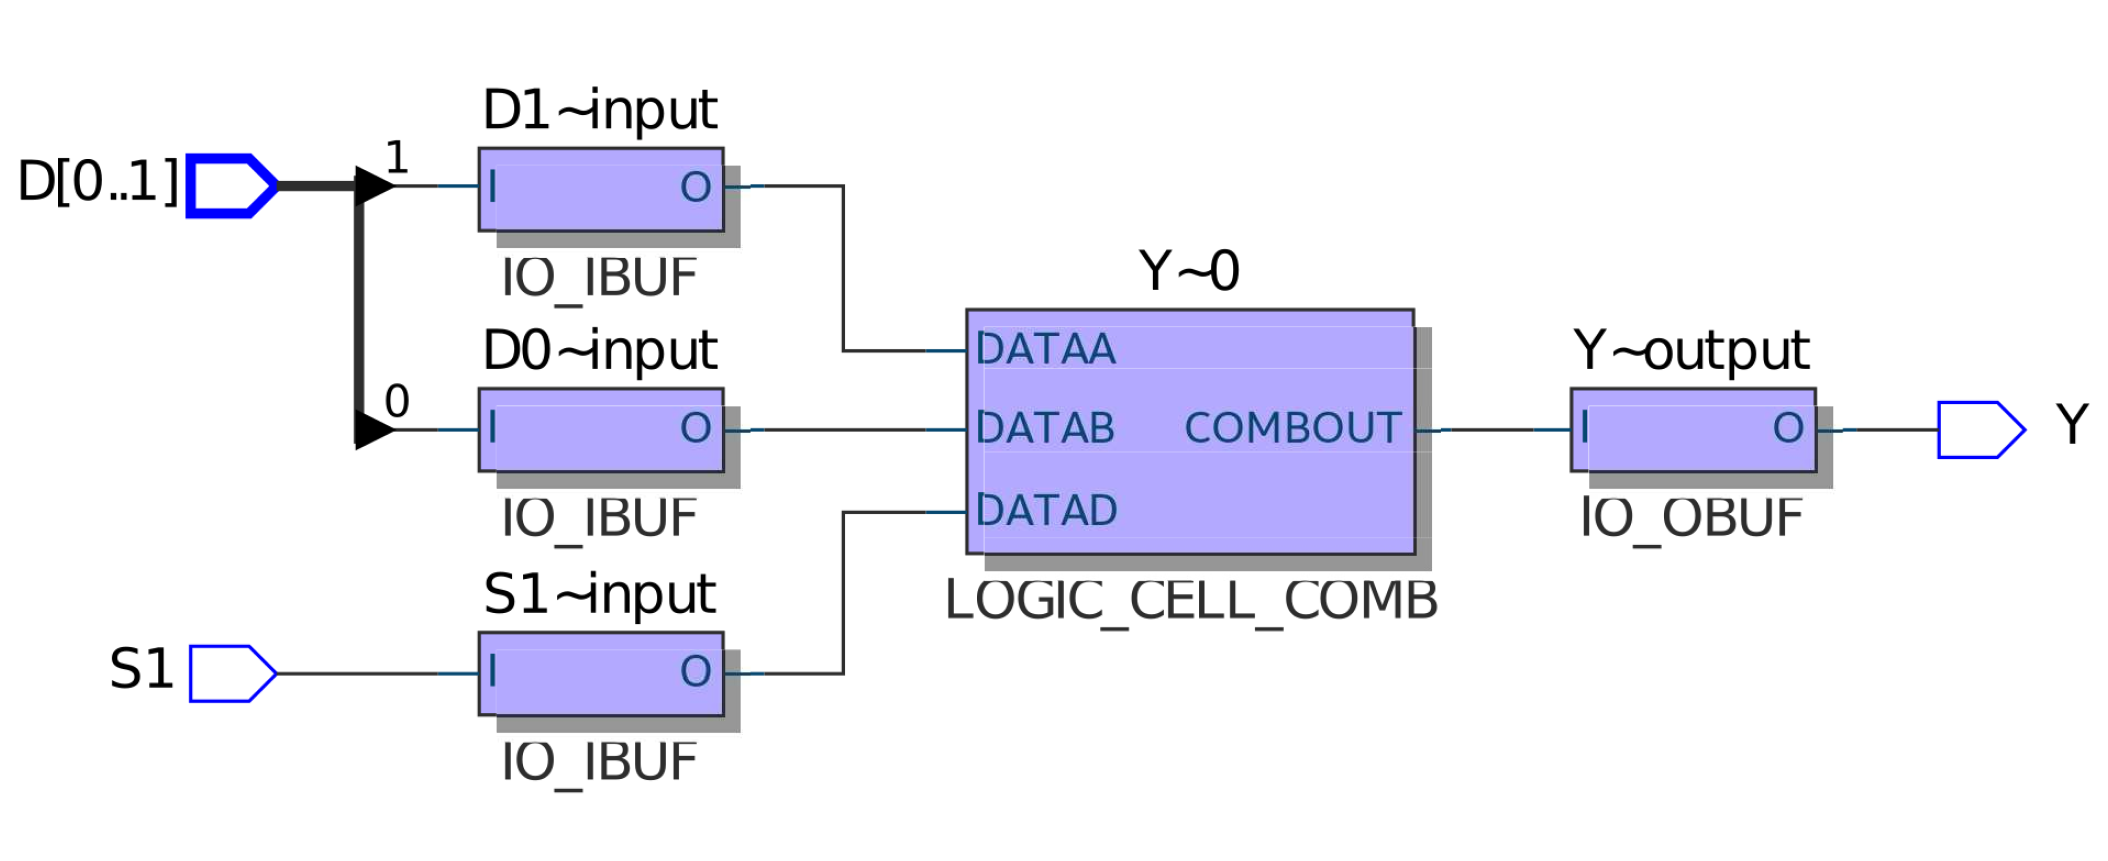
\includegraphics[width=\linewidth]{./src/mux21/mux21_print.png}
  \caption{mux21の回路}
\end{figure}

ロジックエレメント数は2だった。

回路全体の遅延時間は,以下のようになった。
Y~Oの部分で遅延が大きくなった。

\begin{figure}[H]
  \centering
  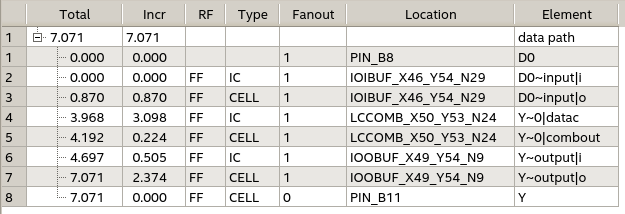
\includegraphics[width=\linewidth]{./src/mux21/mux21Timing.png}
  \caption{mux21の遅延時間}
\end{figure}

\subsubsection{FPGAボードでの動作結果}
スイッチによってS1の値が変わり,それに対応して2つのボタンのうちどちらかの入力がLEDで出力された。

\subsection{考察}
\subsubsection{回路のHDL記述}
コード\ref{mux21.v}では,input output で割り当てた入出力に,assignで単純な論理演算の結果を割り当てている。
Yに$(\lnot{S1} \land D0)|(S1 \land D1)$を割り当てることで,S1の値によってD1とD2のどちらを出力するか選択することができている。
(S1が0の場合D0が,1の場合D1が出力される)

コード\ref{testmux21.v}では,コード\ref{mux21.v}からmux21モジュールを読み込んで動作させながら,20ns間隔で(S1=0, D0=0, D1=0)→(S1=0, D0=1, D1=0)→(S1=1, D0=1, D1=0)→(S1=0, D0=0, D1=0)と入力を遷移させている。

\subsubsection{論理合成}
回路の遅延は,処理が行われているY~Oで大きくなっていた。
実際,以下のようにY~Oにはゲートが配置され,他は入出力用のセルだった 。

\begin{figure}[H]
  \centering
  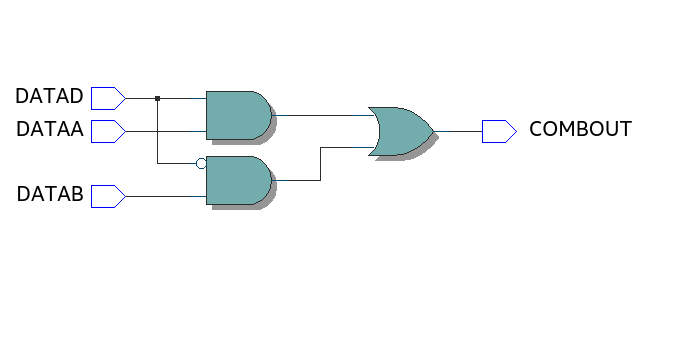
\includegraphics[width=\linewidth]{./src/mux21/mux21elm.png}
  \caption{mux21のゲート}
\end{figure}

また,この結果よりロジックエレメントの値はゲートの数に一致しないことも分かった。\\

この実験で,assign句など,HDL特有の逐次的な動作が理解できた。
また,シュミレータの動作や,論理合成結果の参照が確認できた。


\section{実験2}

\subsection{実験の目的,概要}
本実験では,16ビット加算回路を組み合わせ回路で記述し,機能レベルシュミレーションと論理合成を実行する。
これによって,出力値が仕様を満たしているかどうか,論理合成による回路構成を確認する。

入力は,x,y(16bitオペランド),y(1bit桁上げ入力)。
出力は,sum(16bit演算結果),cout(1bit桁上げ出力)。

ICE計算機上の,ModelSim,Quartusを使用する。

組み合わせ回路の設計法と回路合成結果の確認を目的とする。

\subsection{実験方法}
\subsubsection{回路のHDL記述}
以下のような回路記述をadder16.v,テストベンチをtest\_adder16.vとして作成した。
\lstinputlisting[caption=adder16.v,label=adder16.v]{./src/adder16/adder16.v}
\lstinputlisting[caption=test\_adder16.v,label=testadder16.v]{./src/adder16/test_adder16.v}

\subsubsection{機能レベルシュミレーション}
作成したテストベンチをもとに,ModelSimで信号波形を出力した。
入出力の値が仕様通りの真理値表と一致することを確認した。

\subsubsection{論理合成}
以下の2ファイルを作成し,配置した。
\lstinputlisting[caption=adder16.qpf,label=adder16.qpf]{./src/adder16/adder16.qpf}
\lstinputlisting[caption=adder16.qsf,label=adder16.qsf]{./src/adder16/adder16.qsf}

作成した回路記述をQuartusでコンパイルし,論理合成とレイアウトを行った。
回路構成やロジックエレメント数,遅延時間について確認した。
 
\subsection{実験結果}
\subsubsection{機能レベルシュミレーション}
ModelSimでの入出力波形は以下のようになった。
(キャプチャーでは値が見えないので,赤数字で10進の値を追記した。)

\begin{figure}[H]
  \centering
  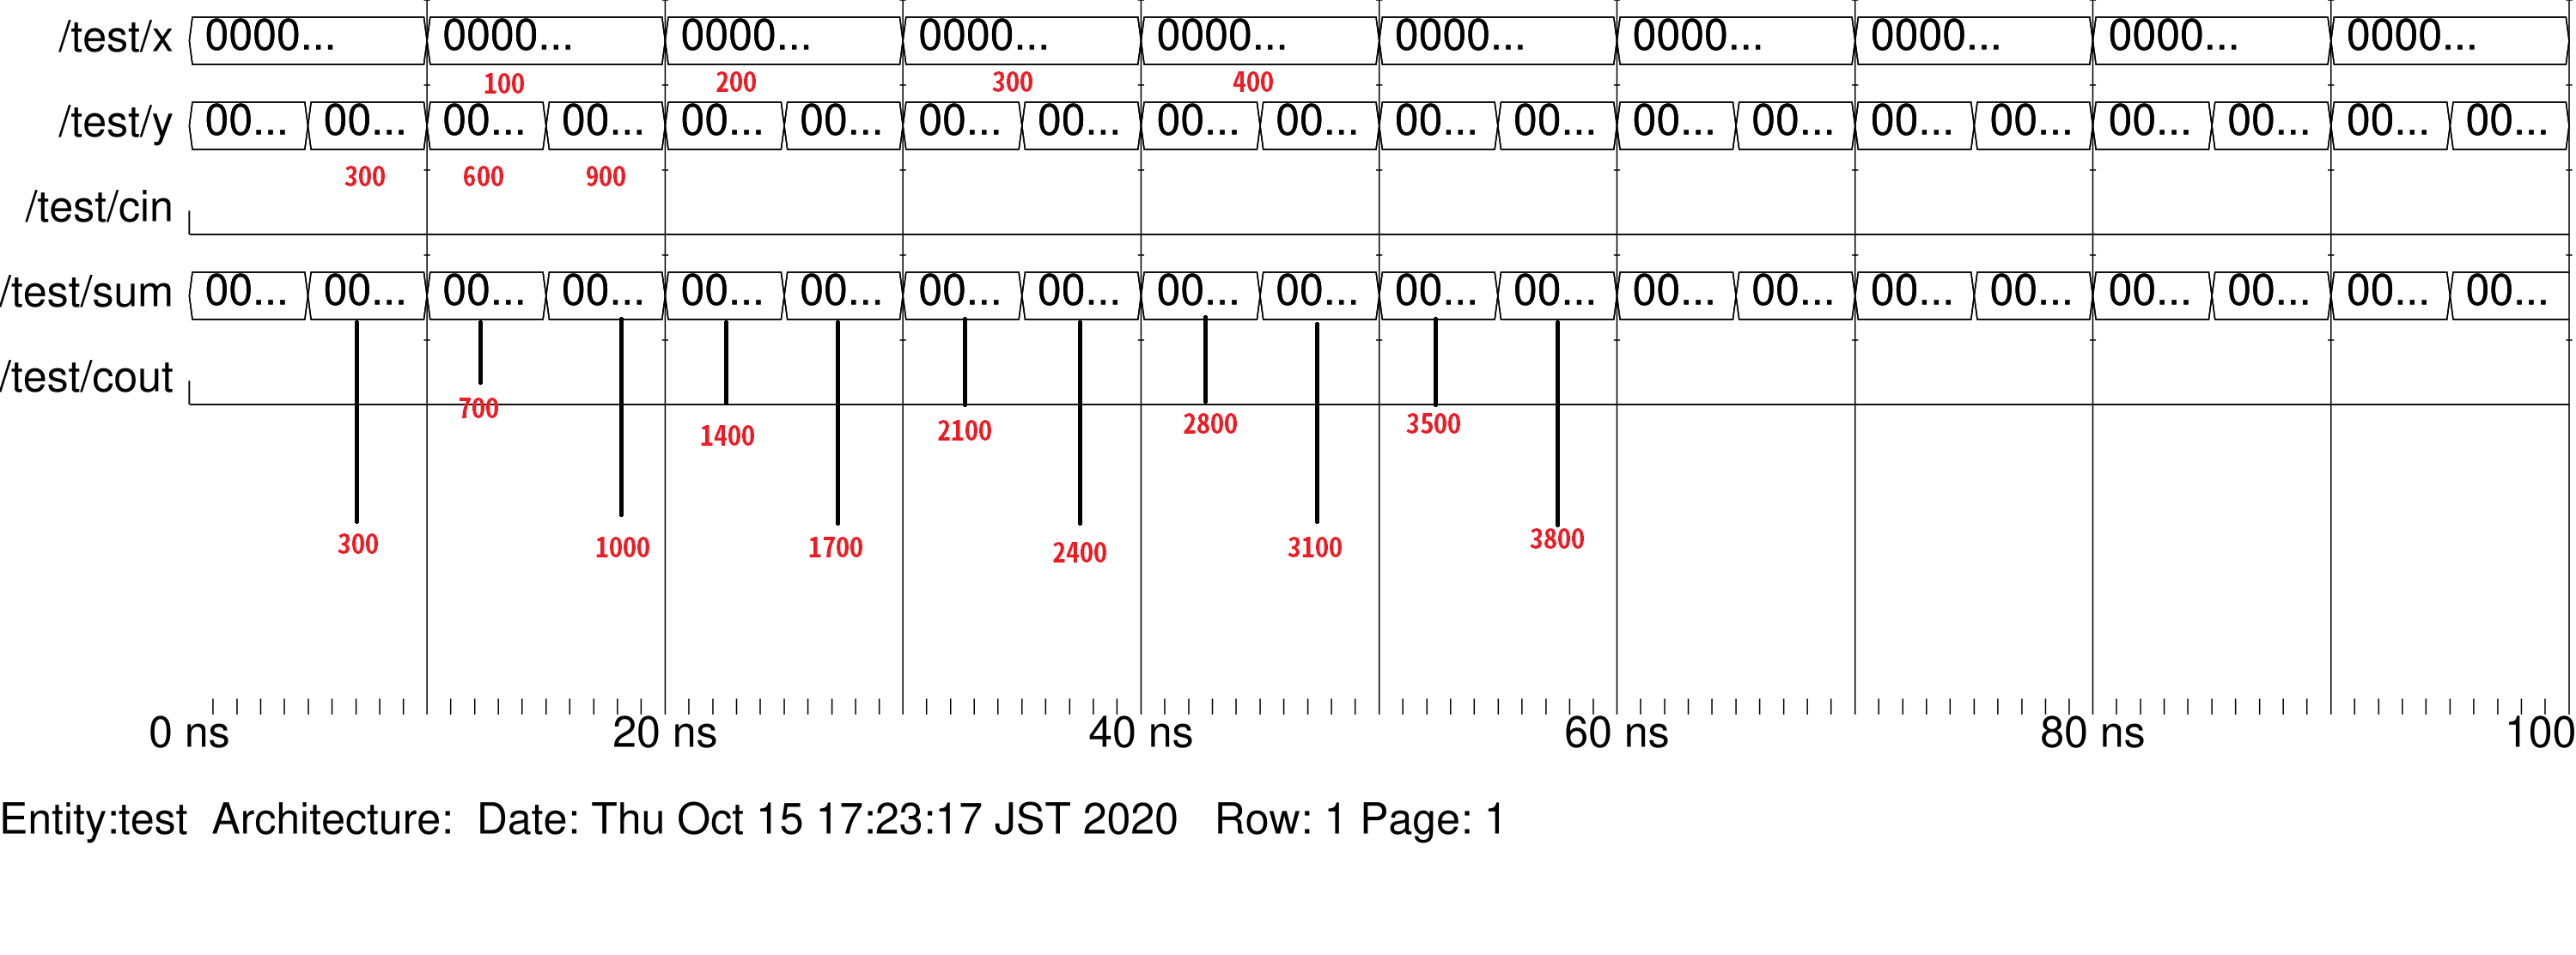
\includegraphics[width=\linewidth]{./src/adder16/adder16_wave21.png}
  \caption{adder16の波形}
\end{figure}

足し算の結果は正しく出力されていることが確認できた。
キャプチャの範囲の外で,coutに桁上げが出力されていることも確認できた。

\subsubsection{論理合成}
論理合成の結果,以下のような回路が作られた。

\begin{figure}[H]
  \centering
  \includegraphics[width=\linewidth]{./src/adder16/adder16_print.png}
  \caption{adder16の回路}
\end{figure}

ロジックエレメント数は19だった。

回路全体の遅延時間は,以下のようになった。

\begin{figure}[H]
  \centering
  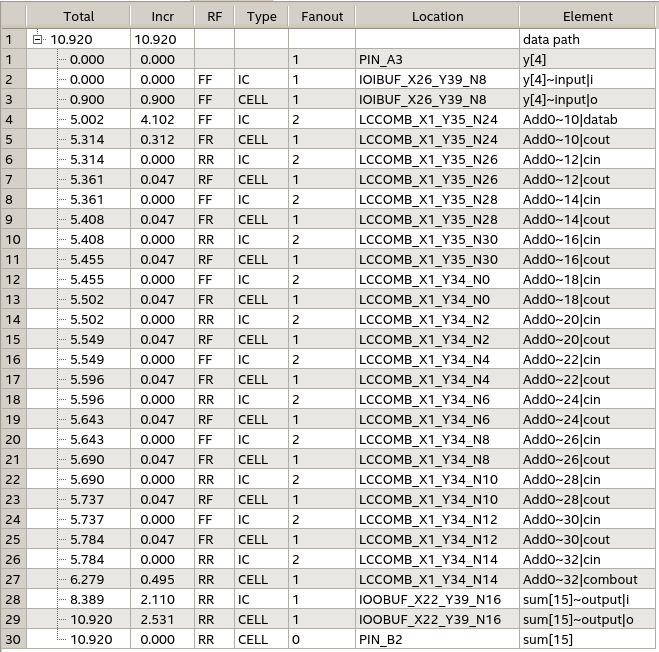
\includegraphics[width=\linewidth]{./src/adder16/adder16Timing.png}
  \caption{adder16の遅延時間}
  \label{adder16の遅延時間}
\end{figure}

\subsection{考察}
\subsubsection{回路のHDL記述}
コード\ref{adder16.v}では,16bitの入出力を定義して,assign句で出力に演算結果を割り当てている。
17bit連接に対して足し算の結果を割り当てているため,結果が16bitに収まらない場合,coutの値は1になる。

コード\ref{testadder16.v}ではテストベンチとして,入力をすべてゼロに初期化し,10nsごとにxを100ずつ加算し,5nsごとにyを300ずつ加算している。

\subsubsection{論理合成}
合成結果より,一桁ごとに桁上りを含めた3入力の全加算器で加算している。
単純な加算機として実装されており,当然桁上りの先読みも行われていないため,そのような記述をすることで,遅延速度が小さくなるのではないかと考える。

遅延時間の表\ref{adder16の遅延時間}より,最長の遅延時間が発生するパスは,最初の全加算器ではなく,(半加算器も含めて)6つめの全加算器への入力から始まっている。
これは,この段階までは配線長とinputIOによる遅延よりも,加算機による遅延のほうが少ないということではないかと予想する。


\section{実験3}
\section{実験3}
\subsection{実験の目的,概要}

\subsection{実験方法}
print\_B.cを編集して,以下のようなファイルmy\_print\_B\_while.cを作成した。
\lstinputlisting[caption=my\_print\_B\_while.c,label=myprintBwhile.c]{./src/obj3/my_print_B_while.c}

以下のコマンドで,MIPS用にクロスコンパイルして,生成されたバイナリからメモリイメージファイルを作成した。

\begin{lstlisting}[caption={クロスコンパイル},label={クロスコンパイル}]
  $ cross_compile.sh my_print_B_while.c
  $ bin2v my_print_B_while.bin
\end{lstlisting}

\subsection{実験結果}
コンパイルの結果,このようなメモリイメージファイルが生成された。
\lstinputlisting[caption=rom8x1024.mif,label=rom8x1024.mif3]{src/obj3/rom8x1024.mif}

内容は,実験2-1で使用したソースコード\ref{rom8x1024.mif2-1}と同じだった。

\subsection{考察}


\section{実験課題1}

\subsection{実験の目的,概要}
1桁のBCDコードを出力するBCDカウンタを設計し,それをもとに2桁のBCDコード出力するBCDカウンタを階層設計によって設計する。
設計した2つの回路で,それぞれ機能レベルシュミレーションと論理合成を実行し,入出力の正しさと合成による結果を確認する。

ICE計算機上の,ModelSim,Quartusを使用する。

この実験で,簡単な順序回路の設計方法と,それをもとにした階層設計の方法を実践し,習得することを目的にする。

\subsection{実験方法}
\subsection*{課題1-1}
\subsubsection{回路のHDL記述}
以下のような回路記述をbcd1.v,テストベンチをtest\_bcd1.vとして作成する。
\lstinputlisting[caption=bcd1.v,label=bcd1.v]{./src/bcd/bcd1.v}
\lstinputlisting[caption=test\_bcd1.v,label=testbcd1.v]{./src/bcd/test_bcd1.v}

\subsubsection{機能レベルシュミレーション}
作成したテストベンチをもとに,ModelSimで信号波形を出力する。
入出力の値が仕様通りの真理値表と一致することを確認する。

\subsubsection{論理合成}
以下の2ファイルを作成し,配置する。
\lstinputlisting[caption=bcd1.qpf,label=bcd1.qpf]{./src/bcd/bcd1.qpf}
\lstinputlisting[caption=bcd1.qsf,label=bcd1.qsf]{./src/bcd/bcd1.qsf}

作成した回路記述をQuartusでコンパイルし,論理合成とレイアウトを行う。回路構成やロジックエレメント数,遅延時間について確認する。

\subsection*{課題1-2}
以下のような回路記述をbcd2.v,テストベンチをtest\_bcd2.vとして作成する。
\lstinputlisting[caption=bcd2.v,label=bcd2.v]{./src/bcd/bcd2.v}
\lstinputlisting[caption=test\_bcd2.v,label=testbcd2.v]{./src/bcd/test_bcd2.v}

\subsubsection{機能レベルシュミレーション}
作成したテストベンチをもとに,ModelSimで信号波形を出力する。
入出力の値が仕様通りの真理値表と一致することを確認する。

\subsubsection{論理合成}
以下の2ファイルを作成し,配置する。
\lstinputlisting[caption=bcd2.qpf,label=bcd2.qpf]{./src/bcd/bcd2.qpf}
\lstinputlisting[caption=bcd2.qsf,label=bcd2.qsf]{./src/bcd/bcd2.qsf}

作成した回路記述をQuartusでコンパイルし,論理合成とレイアウトを行う。回路構成やロジックエレメント数,遅延時間について確認する。

\subsection{実験結果}
\subsection*{課題1-1}
\subsubsection{機能レベルシュミレーション}
ModelSimで波形を作成した結果,以下のような波形になった。

\begin{figure}[H]
  \centering
  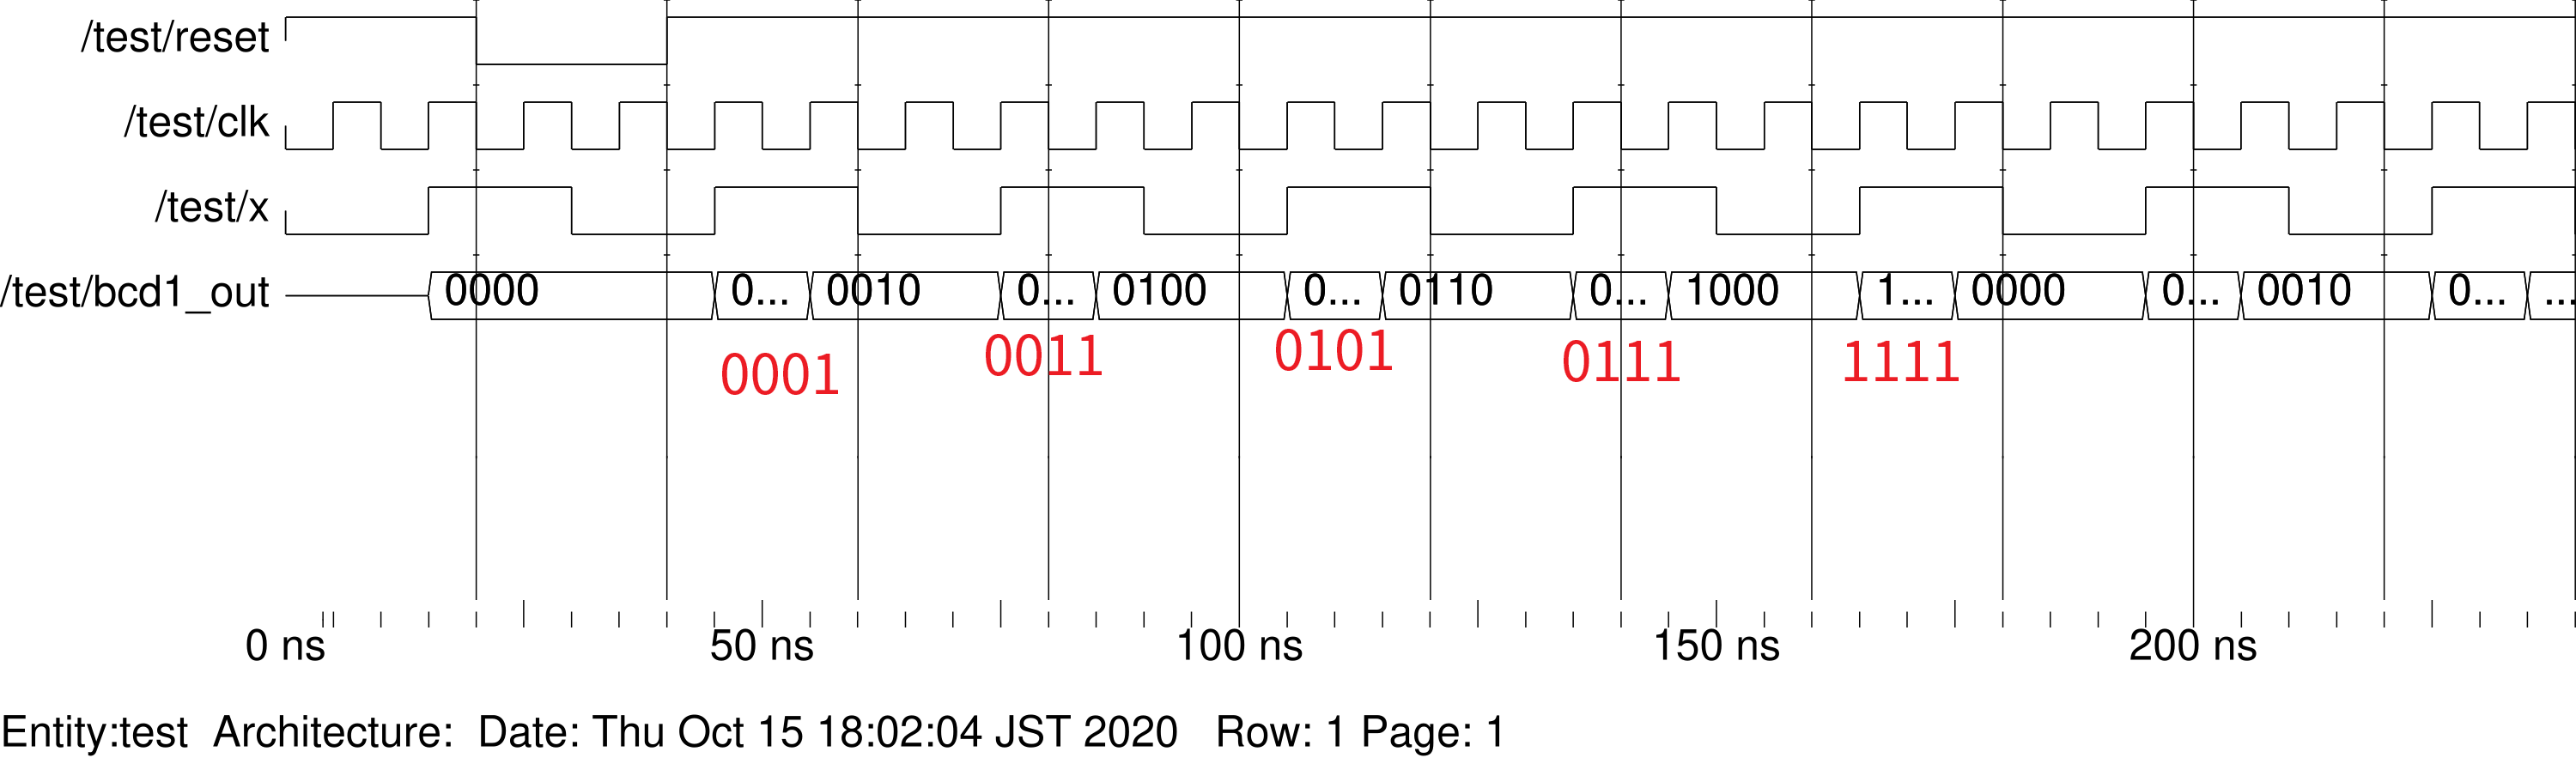
\includegraphics[width=\linewidth]{./src/bcd/bcd1wave.png}
  \caption{bcd1の波形}
\end{figure}

bcd1\_outの値は期待通り10進1桁bcdカウンタとして機能している。

\subsubsection{論理合成}
論理合成の結果,以下のような回路が作られた。

\begin{figure}[H]
  \centering
  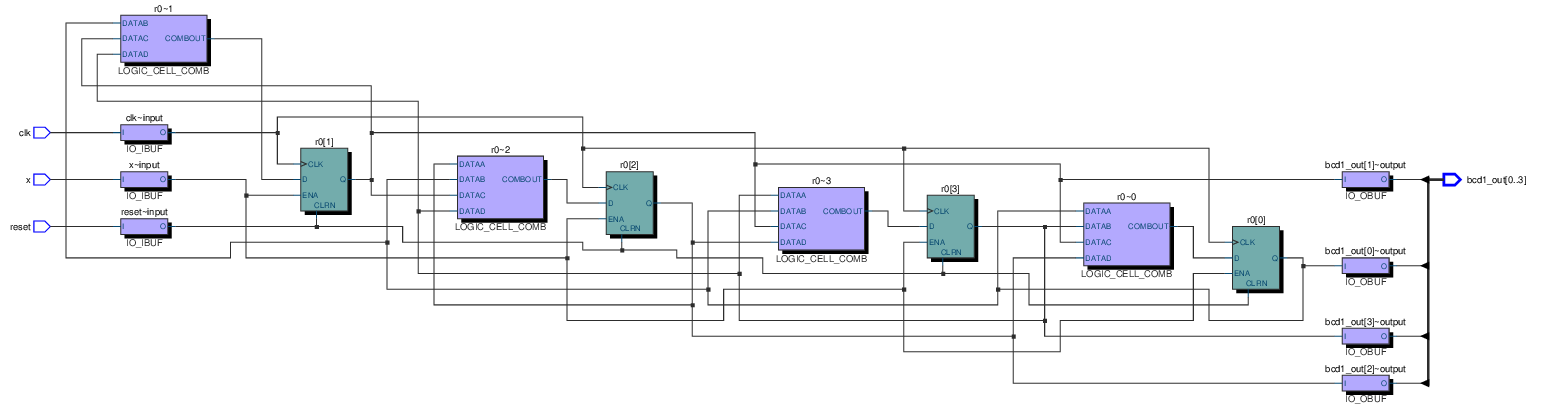
\includegraphics[width=\linewidth]{./src/bcd/bcd1surc.png}
  \caption{bcd1の回路}
\end{figure}

ロジックエレメント数は5だった。

回路全体の遅延時間は,以下のようになった。

\begin{figure}[H]
  \centering
  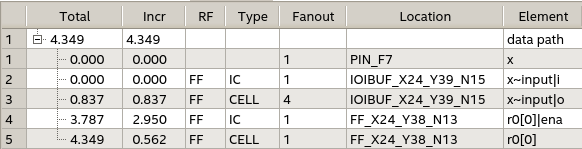
\includegraphics[width=\linewidth]{./src/bcd/bcd1timing.png}
  \caption{bcd1の遅延時間}
\end{figure}

\subsection*{課題1-2}
\subsubsection{機能レベルシュミレーション}
ModelSimで波形を作成した結果,以下のような波形になった。

\begin{figure}[H]
  \centering
  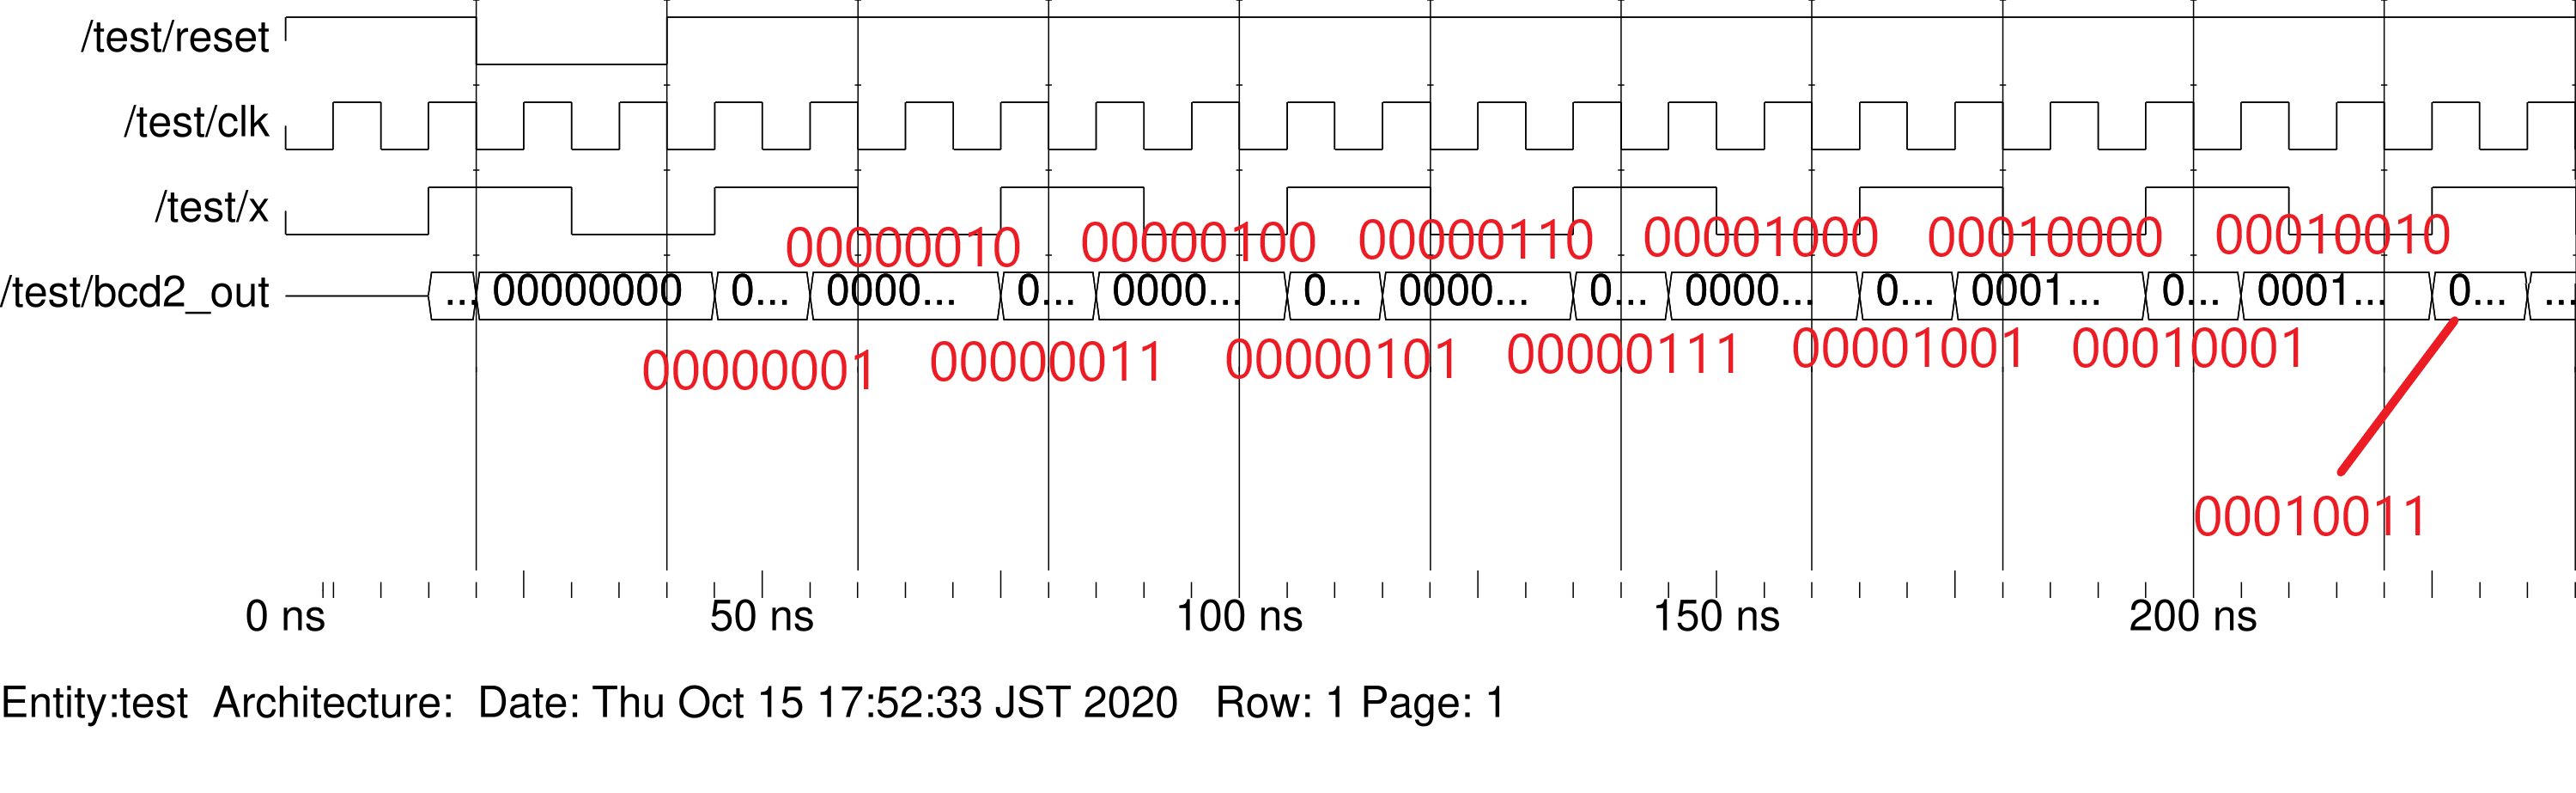
\includegraphics[width=\linewidth]{./src/bcd/bcd2wave.png}
  \caption{bcd2の波形}
  \label{bcd2の波形}
\end{figure}

bcd1\_outの値は期待通り10進2桁bcdカウンタとして機能している。

\subsubsection{論理合成}
論理合成の結果,以下のような回路が作られた。

\begin{figure}[H]
  \centering
  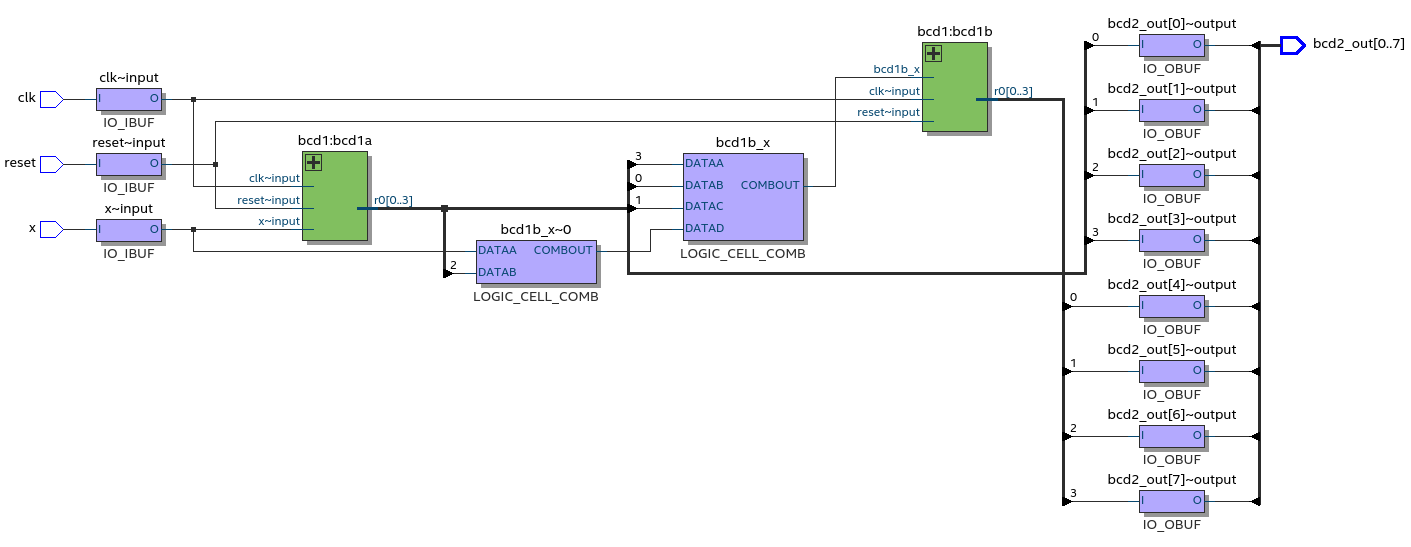
\includegraphics[width=\linewidth]{./src/bcd/bcd2surc.png}
  \caption{bcd2の回路}
  \label{bcd2の回路0}
\end{figure}

bcd1モジュールの他に以下のゲート構成があった。

\begin{figure}[H]
  \centering
  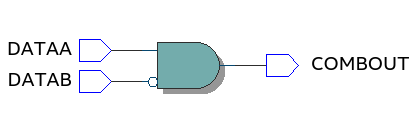
\includegraphics[width=\linewidth]{./src/bcd/bcd2-2x.png}
  \caption{xとbcd1a[2]}
  \label{bcd2の回路1}
\end{figure}

\begin{figure}[H]
  \centering
  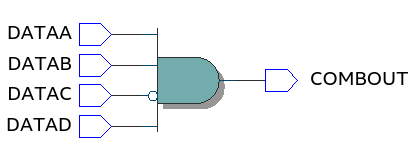
\includegraphics[width=\linewidth]{./src/bcd/bcd2031.png}
  \caption{bcd2[3,0,1]}
  \label{bcd2の回路2}
\end{figure}

ロジックエレメント数は11だった。

回路全体の遅延時間は,以下のようになった。

\begin{figure}[H]
  \centering
  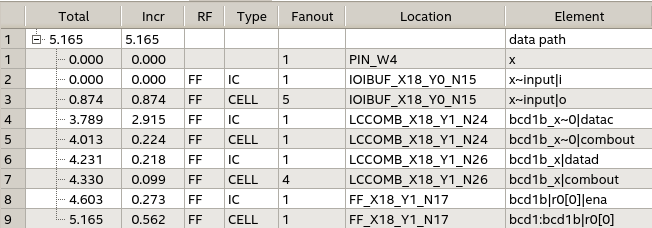
\includegraphics[width=\linewidth]{./src/bcd/bcd2timing.png}
  \caption{bcd2の遅延時間}
\end{figure}

\subsection{考察}
\subsection*{課題1-1}
\subsubsection{回路のHDL記述}
コード\ref{bcd1.v}ではクロックの立ち上がりで,x=1のときに限ってインクリメントしている。
また,レジスタの値が9以上ならば,ゼロを代入している。

リセット信号は,立ち下がりでレジスタにゼロを代入している。

テストベンチ(コード\ref{testbcd1.v})では,5nsごとのクロック反転と,15nsごとのxの反転を実行している。

また,開始20ns後から40ns後までリセット信号を0にしている。

\subsubsection{機能レベルシュミレーション}
1桁のbcdカウンタとして,クロックとxの値によって0~9までの値をとっていた。

\subsubsection{論理合成}
回路では,4桁分のレジスタ用フリップフロップと,各桁での論理演算回路が4桁分あることがわかる。

\subsection*{課題1-2}
\subsubsection{回路のHDL記述}
コード\ref{bcd2.v}では,bcd1のモジュールを利用して2桁分のBCDカウンタを実現している。
具体的には,1桁目が9で桁上りするときに限って,2桁目のBCDカウンタにxを入力している。
また,クロック信号は2つのモジュールに同じ信号を与えている。

リセット信号は,立ち下がりで2つのbcd1モジュールにリセット信号を入力している。

テストベンチ(コード\ref{testbcd2.v})では,5nsごとのクロック反転と,15nsごとのxの反転を実行している。

また,開始20ns後から40ns後までリセット信号を0にしている。

\subsubsection{機能レベルシュミレーション}
図\ref{bcd2の波形}より,4bitを10進1桁分として,2桁分のBCDカウンタが動作している。

\subsubsection{論理合成}
合成された回路では,1桁目の2bit目とxをとって演算した結果を,他のbitと合成して,2桁目のxとして入力していることがわかる。
この部分が,$(bcd1a\_out == 1001) \land x$の結果として反映されていることが分かった。
ほとんど設計したとおりにモジュールが配置されている。

このとき,bcd1モジュールをインラインで展開した場合,回路の構成が異なる可能性がある。
今回の結果より,モジュールの中身については各モジュールで最適化したのと同じ最適化が施されている。
よって,階層設計による回路よりも,インラインで記述したほうがロジックエレメント数や,遅延時間が改善すると予想される。
今回の実験ではわからなかったが,もしそのような差異があるならば,ボード規模などの制限によっては,記述しやすい階層設計と,インラインの記述を使い分ける必要があると予想した。\\

この実験で,順序回路の階層設計の手法と,階層化によって論理合成がどのように行われるかについて理解できた。


\section{実験課題2}

\subsection{実験の目的,概要}
本実験では,0011および0010が入力されるたびに,1を出力する系列検出回路を設計する。
このとき,状態器械による順序回路記述で設計する。
作成した回路は,機能レベルシュミレーションと論理合成を行い,結果を確認する。

ICE計算機上の,ModelSim,Quartusを使用する。

この実験で,オートマトンの設計を回路にどう反映させるかの方法について,習得することを目的にする。

\subsection{実験方法}
\subsubsection{回路のHDL記述}
以下のような回路記述をm.v,テストベンチをtest\_m.vとして作成する。
\lstinputlisting[caption=m.v,label=m.v]{./src/m/m.v}
\lstinputlisting[caption=test\_m.v,label=testm.v]{./src/m/test_m.v}

\subsubsection{機能レベルシュミレーション}
作成したテストベンチをもとに,ModelSimで信号波形を出力する。
入出力の値が仕様通りの真理値表と一致することを確認する。

\subsubsection{論理合成}
以下の2ファイルを作成し,配置する。
\lstinputlisting[caption=m.qpf,label=m.qpf]{./src/m/m.qpf}
\lstinputlisting[caption=m.qsf,label=m.qsf]{./src/m/m.qsf}

作成した回路記述をQuartusでコンパイルし,論理合成とレイアウトを行う。回路構成やロジックエレメント数,遅延時間について確認する。

\subsection{実験結果}
\subsubsection{機能レベルシュミレーション}
ModelSimで波形を作成した結果,以下のような波形になった。

\begin{figure}[H]
  \centering
  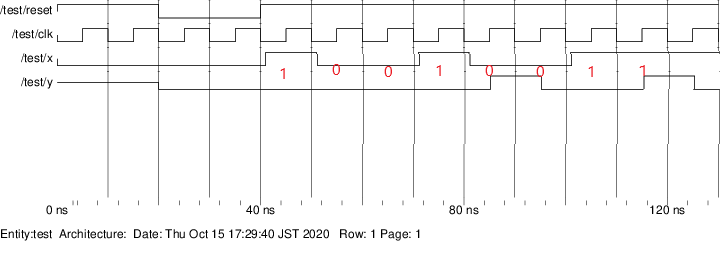
\includegraphics[width=\linewidth]{./src/m/mwave.png}
  \caption{mの波形}
\end{figure}

出力Yは,期待通り2回1を出力していた。

\subsubsection{論理合成}
論理合成の結果,以下のような回路が作られた。

\begin{figure}[H]
  \centering
  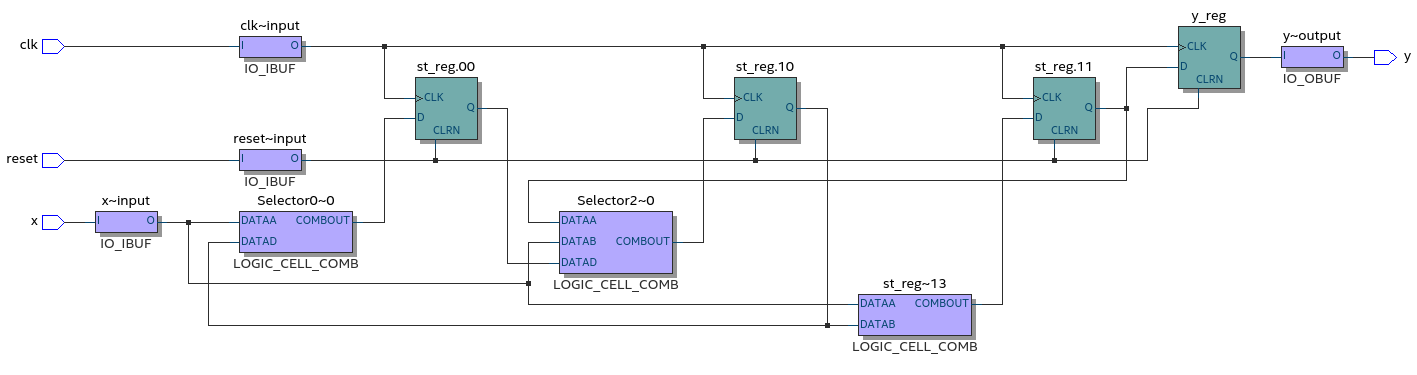
\includegraphics[width=\linewidth]{./src/m/mprint.png}
  \caption{mの回路}
  \label{mの回路}
\end{figure}

ロジックエレメント数は5だった。

回路全体の遅延時間は,以下のようになった。

\begin{figure}[H]
  \centering
  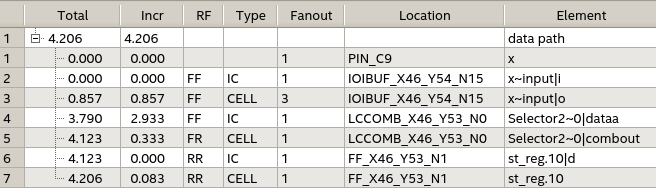
\includegraphics[width=\linewidth]{./src/m/mtiming.png}
  \caption{mの遅延時間}
\end{figure}

\subsection{考察}
\subsubsection{回路のHDL記述}
図\ref{設計したオートマトン}のような出力付きのオートマトンをもとにして,回路記述を行った。
レジスタに状態を記憶し,入力に応じて状態を遷移,出力する。

今回は,0010011のような系列に2回検出を行うオートマトンを設計した。

\begin{figure}[H]
  \centering
  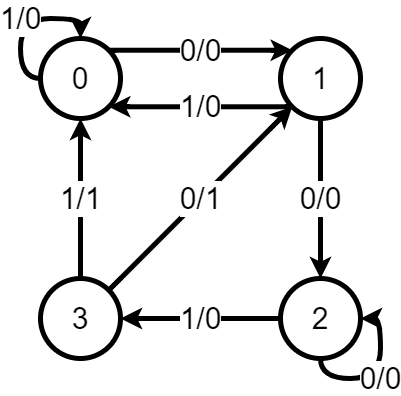
\includegraphics[width=5cm]{./src/m/mautomaton.png}
  \caption{設計したオートマトン}
  \label{設計したオートマトン}
\end{figure}

\subsubsection{機能レベルシュミレーション}
テストベンチでは,これまでの順序回路と同様な設定の後に,1→0→0→1→0→0→1→1という系列を10nsおきに入力している。
最初に0010が,次に0011が検出されることが期待されて,実際に2回検出されている。

\subsubsection{論理合成}
コード\ref{m.v}では,4状態のオートマトンと出力レジスタが宣言されているが,図\ref{mの回路}では,合成によって3つの状態と出力,論理演算のみで構成されていることがわかった。
状態として持っていた情報を,現在の状態と入力の演算として再定義することで,状態数を削減しているのだと予想する。\\

この実験で,オートマトンの設計を順序回路として記述する方法がわかった。
また,そのような回路は合成によって状態数が減ることがある,ということも確認できた。


\section{論理合成の最適化について}
\subsection{具体的な手法}
HDLで記述された回路は,まず論理演算等が率直に実装される。
次に,各演算に対する最適化や,モジュールの共用が行われる。

具体的には,カルノー図による論理関数の簡単化や,1ゲートで実行できる演算の置換が行われる(XORなど)。

モジュールの共用では,次のような最適化例がある。
2入力1出力の,入力をゲートAに通してゲートBに通す回路を考える。
このとき,素の入力にゲートBを施してからゲートAを通す回路が,等価な回路として考えられる場合,ゲートの数を1つ削減することができる。

ZHANG, ZHIFEI\cite{RTL}によると,HDL記述の抽象度が高いほど,このような最適化を行う余地が生まれ,回路規模も遅延も小さくなる傾向があるとされている。
実際,実験2で桁上りの先読みについて予想しているが,ZHANG, ZHIFEI\cite{RTL}では回路規模の点でも配線長の点でも不利になることから,4bit加算器の場合は,ナイーブな実装のほうが優れているとされている。

\subsection{遅延時間と回路面積の関係}
ALTERA\cite{ALTERA}によると,回路合成による回路の分散と遅延時間はトレードオフになっていることがわかる。
しかし,面積が小さい場合,配線の長さによる遅延時間も大きくなり,ZHANG, ZHIFEI\cite{RTL}のキャリー読み加算回路のように,配線前後で遅延時間が大幅に変動する。

つまり,最適化の結果,段数を増やしてクリティカルパスを短くするような回路では,面積と遅延がトレードオフになる。
しかし,演算による遅延に対して配線の影響が大きい場合,遅延は面積の大きさに伴って増加する。

\begin{thebibliography}{99}
  \bibitem{ALTERA}AN 584: 高度な FPGA デザインにおける  タイミング・クロージャ手法, ALTERA,\url{https://www.intel.co.jp/content/dam/altera-www/global/ja_JP/pdfs/literature/an/an584.pdf}
  \bibitem{RTL} RTLとゲートレベルを混在させた最適な論理回路設計に関する研究,ZHANG, ZHIFEI,\url{https://dspace.jaist.ac.jp/dspace/handle/10119/12013}
\end{thebibliography}
すべて2020年10月22日閲覧

\end{document}
